\documentclass{article}
\usepackage{amsthm}
\usepackage{amsmath}
\usepackage{amsfonts}
\usepackage{amssymb}
\usepackage[utf8]{inputenc}
\usepackage{titling}
\usepackage{scrextend}
\usepackage{graphicx}

\title{Real Analysis II - Homework II}
\author{Lucas LaValva}
\date{\today}

\usepackage{fancyhdr}
\pagestyle{fancy}
\lhead{\theauthor}
\rhead{\thetitle}

\begin{document}
\maketitle

\setcounter{section}{5}

\section{Series of Functions}

\subsection{Lim sup and Lim inf}
\begin{enumerate}
      \setcounter{enumi}{1}
      \item Let $a_n=1$ if $n=2^k$ for some positive integer $k$,
            and $a_n=\frac{1}{n!}$ otherwise.
            \begin{enumerate}
                  \item Find $\limsup a_n$ and $\liminf a_n$.
                        \begin{proof}
                              Let $\bar s=1$ and $\varepsilon>0$ be given.
                              Then choose any $N>0$.
                              It follows that, for all $n>N$,
                              \begin{align*}
                                    a_n & = \begin{cases}
                                          1            & n=2^k      \\
                                          \frac{1}{n!} & n \neq 2^k
                                    \end{cases}    \\
                                        & \leq \begin{cases}
                                          1 & n=2^k      \\
                                          1 & n \neq 2^k
                                    \end{cases} \\
                                        & = 1                            \\
                                        & = \bar s                       \\
                                        & \leq \bar s + \varepsilon.
                              \end{align*}
                              Moreover, for any selected $N$ we can choose
                              $n_o=2^N$ so that
                              \begin{align*}
                                    a_{n_o} & = 1                        \\
                                            & = \bar s                   \\
                                            & \geq \bar s - \varepsilon.
                              \end{align*}
                              Therefore, $\limsup a_n=1$.
                        \end{proof}
                        \begin{proof}
                              Let $\underline{s}=0$ and $\varepsilon>0$ be given.
                              Then choose $N>\frac{1}{\varepsilon}$.
                              It follows that, for all $n>N$,
                              \begin{align*}
                                    a_n & = \begin{cases}
                                          1            & n=2^k      \\
                                          \frac{1}{n!} & n \neq 2^k
                                    \end{cases}     \\
                                        & \geq \begin{cases}
                                          \frac{1}{n!} & n=2^k      \\
                                          \frac{1}{n!} & n \neq 2^k
                                    \end{cases}  \\
                                        & = \frac{1}{n!}                  \\
                                        & \geq 0                          \\
                                        & = \underline{s}                 \\
                                        & \geq \underline{s}-\varepsilon.
                              \end{align*}
                              Moreover, for any selected $N$ we can choose
                              $n_o=2^N+1$ so that
                              \begin{align*}
                                    a_{n_o} & = \frac{1}{n_o!}             \\
                                            & \leq \frac{1}{n_o}           \\
                                            & \leq \frac{1}{N}             \\
                                            & \leq \varepsilon             \\
                                            & = 0 + \varepsilon            \\
                                            & = \underline{s}+\varepsilon.
                              \end{align*}
                              Therefore, $\liminf a_n=0$.
                        \end{proof}
                  \item Find $\limsup\frac{\lvert a_{n+1}\rvert}{\lvert a_n\rvert}$.
                        \begin{proof}
                              Let $b_n=\frac{\lvert a_{n+1}\rvert}{\lvert a_n\rvert}$
                              and $n_k=2^k-1$. Then
                              \begin{align*}
                                    b_{n_k} & = \frac{\lvert a_{n_k+1}\rvert}{\lvert a_{n_k}\rvert} \\
                                            & = \frac{a_{2^k}}{a_{2^k-1}}                           \\
                                            & = \frac{1}{\frac{1}{(2^k-1)!}}                        \\
                                            & = (2^k-1)!                                            \\
                                            & = n_k!
                              \end{align*}
                              Which is clearly divergent. Since $b$ has a divergent
                              subsequence, it must be divergent in the sup norm.
                              Therefore $\limsup b_n = \infty$.
                        \end{proof}
                  \item Find $\limsup\lvert a_n\rvert^\frac{1}{n}$.
                        \begin{proof}
                              Let $\bar s = 1$ and $\varepsilon>0$ be given.
                              Then for any $N>0$,
                              it follows that for all $n>N$,
                              \begin{align*}
                                    \lvert a_n\rvert^\frac{1}{n} & = \begin{cases}
                                          \lvert 1\rvert^\frac{1}{n}           & n=2^k      \\
                                          \lvert\frac{1}{n!}\rvert^\frac{1}{n} & n \neq 2^k
                                    \end{cases} \\
                                                                 & = \begin{cases}
                                          1                      & n=2^k      \\
                                          \sqrt[n]{\frac{1}{n!}} & n \neq 2^k
                                    \end{cases} \\
                                                                 & \leq 1                      \\
                                                                 & = \bar s                    \\
                                                                 & \leq \bar s + \varepsilon.
                              \end{align*}
                              Moreover, it can be shown that, for $n_o=2^N$,
                              \begin{align*}
                                    a_{n_o} & = 1                        \\
                                            & = \bar s                   \\
                                            & \geq \bar s - \varepsilon.
                              \end{align*}
                              Therefore, $\limsup\lvert a_n\rvert^\frac{1}{n} = \bar s = 1$.
                        \end{proof}
            \end{enumerate}
            \setcounter{enumi}{4}
      \item Let $\{a_n\}$ be a sequence of real numbers and suppose
            that $\limsup a_n$ is finite. Let $\{c_n\}$ be another
            sequence and suppose that $c_n\to c$.
            \begin{enumerate}
                  \item Prove that, if $c>0$, then
                        \begin{equation}
                              \limsup c_na_n = c\limsup a_n.
                              \label{eq:6.1_5_given}
                        \end{equation}
                        \begin{proof}
                              Let $\varepsilon>0$ be given, and
                              $\varepsilon'=\frac{\varepsilon}{2\left(\bar s_a + c\right)}$.
                              Since $\limsup a_n$ is finite, we know there exists
                              some $\bar s_a\in \mathbb{R}$ and $N_a>0$ so that for all $n>N_a$,
                              \[
                                    a_n \leq \bar s_a + \varepsilon'
                              \]
                              and there exists some $n_o>N_a$ so that
                              \[
                                    a_{n_o} \geq \bar s_a - \varepsilon'.
                              \]
                              We also know that, because $c_n\to c$, there exists
                              $N_c>0$ so that for all $n>N_c$,
                              \begin{align*}
                                    \lvert c_n-c\rvert & < \varepsilon'.    \\
                                    c_n                & < c + \varepsilon' \\
                                    c_n                & > c - \varepsilon'
                              \end{align*}
                              Let $N=\max(N_a, N_c)$. Then it follows that, for all
                              $n>N$,
                              \begin{align*}
                                    c_na_n & \leq \left(c + \varepsilon'\right)\left(\bar s_a + \varepsilon'\right)                                                                 \\
                                           & = c\bar s_a + \left(c+\bar s_a\right)\varepsilon' + \varepsilon'^2                                                                     \\
                                           & = c\bar s_a + \left(c+\bar s_a\right)\frac{\varepsilon}{2\left(\bar s_a + c\right)} + \frac{\varepsilon}{2\left(\bar s_a + c\right)}^2 \\
                                           & = c\bar s_a + \frac{\varepsilon}{2} + \frac{\varepsilon}{2}^2                                                                          \\
                                    c_na_n & \leq c\bar s_a + \varepsilon
                              \end{align*}
                              and there exists some $n_o>N$ so that
                              \begin{align*}
                                    c_{n_o}a_{n_o} & \geq \left(c - \varepsilon'\right)\left(\bar s_a - \varepsilon'\right)                                                                 \\
                                                   & = c\bar s_a - \left(c+\bar s_a\right)\varepsilon' + \varepsilon'^2                                                                     \\
                                                   & = c\bar s_a - \left(c+\bar s_a\right)\frac{\varepsilon}{2\left(\bar s_a + c\right)} + \frac{\varepsilon}{2\left(\bar s_a + c\right)}^2 \\
                                                   & = c\bar s_a - \frac{\varepsilon}{2} + \frac{\varepsilon}{2}^2                                                                          \\
                                    c_{n_o}a_{n_o} & \geq c\bar s_a - \varepsilon
                              \end{align*}
                              Therefore, $\limsup c_na_n = c\bar s_a = c\limsup a_n$.
                        \end{proof}
                  \item Find a counterexample to \eqref{eq:6.1_5_given}
                        with $c<0$.
                        \begin{proof}
                              Let $a_n=2\sin(n)+1$ and $c_n=-1$. Then $\limsup a_n=3$
                              and $c=-1$. However, $a_nc_n=-2\sin(n)-1$ and thus
                              $\limsup a_nc_n=1$. Therefore,
                              \begin{align*}
                                    \limsup a_nc_n & = 1               \\
                                    c\limsup a_n   & = -3              \\
                                    1              & \neq -3           \\
                                    \limsup a_nc_n & \neq c\limsup a_n
                              \end{align*}
                              Alas! \eqref{eq:6.1_5_given} is not always true when $c<0$
                        \end{proof}
            \end{enumerate}
            \setcounter{enumi}{8}
      \item Let $\{a_n\}$ be a bounded sequence of real numbers and
            let $P$ be the set of limit points of $\{a_n\}$. Limit
            points are defined in Section 2.6. Prove that
            $\limsup a_n=\sup P$ and $\liminf a_n=\inf P$.
            \begin{proof}
                  The Bolzano-Weierstrass theorem tells us that $\{a_n\}$ must
                  have one or more convergent subsequences. By definition, $P$
                  contains the limits of each of these convergent subsequences.
                  Then for all subsequences $a_{n_k}$ of $a_n$ and $\varepsilon>0$,
                  \begin{align*}
                        \lim a_{n_k} - \sup P & \leq \varepsilon           \\
                        \lim a_{n_k}          & \leq \sup P + \varepsilon.
                  \end{align*}
                  Because all points on $P$ are limits of subsequences of $a_n$,
                  there must also exist some $a_{n_s}$ so that
                  \begin{align*}
                        \lvert\lim a_{n_s} - \sup P\rvert & \leq \varepsilon           \\
                        \lim a_{n_s} - \sup P             & \geq -\varepsilon          \\
                        \lim a_{n_s}                      & \geq \sup P - \varepsilon.
                  \end{align*}
                  Therefore, $\limsup a_n=\sup P$.
                  \medbreak
                  We also know that
                  \begin{align*}
                        \lim a_{n_k} - \inf P & \geq -\varepsilon         \\
                        \lim a_{n_k}          & \leq \inf P - \varepsilon
                  \end{align*}
                  and that there exists some $a_{n_i}$ so that
                  \begin{align*}
                        \lvert\lim a_{n_i} - \inf P\rvert & \leq \varepsilon           \\
                        \lim a_{n_i} - \inf P             & \leq \varepsilon           \\
                        \lim a_{n_i}                      & \geq \inf P + \varepsilon.
                  \end{align*}
                  Thus, $\liminf a_n=\inf P$.
            \end{proof}
\end{enumerate}

\subsection{Series of Real Constants}
\begin{enumerate}
      \item Determine whether the following series converge
            or diverge:
            \begin{enumerate}
                  \item $\sum\frac{3^j}{j!}$
                        \begin{proof}[Converges.]
                              By the ratio test,
                              \begin{align*}
                                    \limsup \frac{a_{j+1}}{a_j} & = \limsup \frac{\frac{3^{j+1}}{(j+1)!}}{\frac{3^j}{j!}} \\
                                                                & = \limsup \frac{3^{j+1}(j!)}{3^j(j+1)!}                 \\
                                                                & = \limsup \frac{3(3^j)j!}{3^j(j+1)j!}                   \\
                                                                & = \limsup \frac{3}{j+1}                                 \\
                                    \frac{3}{j+1}               & < 1 \textrm{ for all $j>2$, so}                         \\
                                    \limsup \frac{3}{j+1}       & < 1
                              \end{align*}
                        \end{proof}
                  \item $\sum\frac{\sqrt{n}}{1+n^2}$
                        \begin{proof}[Converges.]
                              By the comparison test,
                              \begin{align*}
                                    a_n & = \frac{\sqrt{n}}{1+n^2}       \\
                                        & \leq \frac{n^\frac{1}{2}}{n^2} \\
                                        & = \frac{1}{n^\frac{3}{2}},
                              \end{align*}
                              which is a convergent $p$-series because $p>1$
                        \end{proof}
                  \item $\sum\frac{2^j}{j^2}$
                        \begin{proof}[Diverges.]
                              By the ratio test,
                              \begin{align*}
                                    \frac{a_{j+1}}{a_j}                    & = \frac{\frac{2^{j+1}}{(j+1)^2}}{\frac{2^j}{j^2}}        \\
                                                                           & = \frac{2^{j+1}j^2}{2^j(j+1)^2}                          \\
                                                                           & = \frac{2j^2}{(j+1)^2}                                   \\
                                                                           & \geq \frac{2j^2}{\frac{3}{2}j^2} \textrm{ for all $j>5$} \\
                                                                           & = \frac{4}{3}                                            \\
                                    \therefore \liminf \frac{a_{j+1}}{a_j} & \geq \frac{4}{3} > 1
                              \end{align*}
                        \end{proof}
                  \item $\sum\frac{j^2}{j!}$
                        \begin{proof}[Converges.]
                              By the ratio test,
                              \begin{align*}
                                    \frac{a_{j+1}}{a_j}                  & = \frac{\frac{(j+1)^2}{(j+1)!}}{\frac{j^2}{j!}} \\
                                                                         & = \frac{(j+1)^2j!}{j^2(j+1)j!}                  \\
                                                                         & = \frac{j^2+2j+1}{j^3+j^2}                      \\
                                                                         & \leq \frac{j^2}{j^3}+\frac{2j}{j^2}+\frac{1}{j} \\
                                                                         & = \frac{4}{j}                                   \\
                                                                         & < 1 \textrm{ for all $j>4$}                     \\
                                    \therefore\limsup\frac{a_{j+1}}{a_j} & < 1
                              \end{align*}
                        \end{proof}
                  \item $\sum(\sqrt{j+1}-\sqrt{j})$
                        \begin{proof}[Diverges.]
                              This is a telescoping series, expanded as
                              \begin{align*}
                                    \sum_{j=0}^k(\sqrt{j+1}-\sqrt{j}) & = \sqrt{1}-\sqrt{0}+\sqrt{2}-\sqrt{1}+\ldots+\sqrt{k+1}-\sqrt{k}     \\
                                                                      & = -\sqrt{0}+(\sqrt{1}-\sqrt{1})+\ldots(\sqrt{k}-\sqrt{k})+\sqrt{k+1} \\
                                                                      & = \sqrt{k+1}
                              \end{align*}
                              As $k$ grows to $\infty$, $\sqrt{k+1}$ also grows to $\infty$.
                              Therefore, the series diverges.
                        \end{proof}
                  \item $\sum\frac{\sqrt{j+1}-\sqrt{j}}{j}$
                        \begin{proof}[Converges.]
                              By the comparison test,
                              \begin{align*}
                                    \frac{\sqrt{j+1}-\sqrt{j}}{j} & = \frac{(\sqrt{j+1}-\sqrt{j})(\sqrt{j+1}+\sqrt{j})}{j(\sqrt{j+1}+\sqrt{j})} \\
                                                                  & = \frac{j+1-j}{j(\sqrt{j+1}+\sqrt{j})}                                      \\
                                                                  & \leq \frac{1}{2j\sqrt{j}}                                                   \\
                                                                  & = \frac{1}{2j^{\frac{3}{2}}}
                              \end{align*}
                              which is a $p$-series with $p>1$, so the series is convergent.
                        \end{proof}
                  \item $\sum e^{-j+\sin j}$
                        \begin{proof}[Converges.]
                              By the comparison test,
                              \begin{align*}
                                    e^{-j+\sin j} & = \frac{e^{\sin j}}{e^j} \\
                                                  & \leq \frac{e}{e^j}
                              \end{align*}
                              and
                              \begin{align*}
                                    \sum \frac{e}{e^j} & = e\sum \frac{1}{e^j}               \\
                                                       & = e\sum \left(\frac{1}{e}\right)^j.
                              \end{align*}
                              This is a power series, which converges because the power term is less than 1.
                              Therefore, the series converges.
                        \end{proof}
                  \item $\sum\frac{j+\cos j}{j}$
                        \begin{proof}[Diverges.]
                              It is clear that
                              \begin{align*}
                                    \sum\frac{j+\cos j}{j} & = \sum\left(\frac{j}{j} + \frac{\cos j}{j}\right) \\
                                                           & = \sum(1) + \sum\left(\frac{\cos j}{j}\right).
                              \end{align*}
                              Without a doubt, $\sum(1)$ is divergent and therefore the series is divergent.
                        \end{proof}
            \end{enumerate}
            \setcounter{enumi}{3}
      \item Consider the series $\sum_{j=1}^\infty\frac{1}{j(j+1)}$.
            \begin{enumerate}
                  \item Prove that the series converges by the
                        comparison test
                        \begin{proof}
                              By the comparison test,
                              \begin{align*}
                                    \frac{1}{j(j+1)} & \leq \frac{1}{j(j)} \\
                                                     & = \frac{1}{j^2}
                              \end{align*}
                              which is a $p$-series with $p>1$, so the series converges.
                        \end{proof}
                  \item What information does the ratio test give?
                        \begin{align*}
                              \frac{a_{j+1}}{a_j} & = \frac{\frac{1}{(j+1)(j+2)}}{\frac{1}{j(j+1)}} \\
                                                  & = \frac{j(j+1)}{(j+1)(j+2)}                     \\
                                                  & = \frac{j}{j+2}
                        \end{align*}
                        INCONCLUSIVE, $\lim\frac{j}{j+2}=1$.
                  \item Use the formula $\frac{1}{j(j+1)}=\frac{1}{j}-\frac{1}{j+1}$
                        to compute the partial sums. Show explicitly that
                        the partial sums converge.
                        \begin{align*}
                              \sum_{j=1}^k \left(\frac{1}{j}-\frac{1}{j+1}\right) & = \frac{1}{1}-\frac{1}{2}+\frac{1}{2}-\frac{1}{3}+\ldots+\frac{1}{k}-\frac{1}{k+1}                               \\
                                                                                  & = 1 + (\frac{1}{2}-\frac{1}{2}) + (\frac{1}{3}-\frac{1}{3}) + \ldots + (\frac{1}{k}-\frac{1}{k}) - \frac{1}{k+1} \\
                                                                                  & = 1 - \frac{1}{k+1}
                        \end{align*}
                        This series approaches $1$ as $k$ approaches infinity.
            \end{enumerate}
            \setcounter{enumi}{12}
      \item Prove that if $a_j\geq 0$ for all $j$ and $\sum a_j$
            converges, then $\sum a_j^2$ converges.
            \begin{proof}
                  We know that, because all $a_j\geq 0$ and the sequence converges,
                  there exists some $J$ for each $\varepsilon$ so that
                  $\sum_{j=J}^\infty \lvert a_j\rvert < \varepsilon$. Without loss of generality,
                  we can assume that $\varepsilon<1$. Then for all $j>J$, $a_j<1$. This
                  tells us that for all $j>J$, $a_j^2<a_j$ and thus
                  $\sum_{j=J}^\infty a_j^2 < \sum_{j=J}^\infty \lvert a_j\rvert < \varepsilon$.
                  Therefore, $\sum a_j^2$ converges.
            \end{proof}
      \item Suppose that $a_j\geq 0$ and that $\sum a_j$ converges.
            \begin{enumerate}
                  \item Show by example that it is not necessarily true that
                        $\sum\sqrt{a_j}$ converges.
                        \begin{proof}
                              Let $a_j=\frac{1}{j^2}$. Then $\sum a_j$ is a convergent
                              $p$-series, with $p>1$. However, in this case
                              $\sum\sqrt{a_j}$ is the harmonic series, which is not
                              convergent.
                        \end{proof}
                  \item Show that $\sum\frac{\sqrt{a_j}}{j}$ converges.
                        % TODO: This one is hard
            \end{enumerate}
\end{enumerate}

\subsection{The Weierstrass M-test}

\begin{enumerate}
      \setcounter{enumi}{2}
      \item \begin{enumerate}
                  \item Prove that $\sum_{j=0}^\infty x^j$ is differentiable
                        on $(0,1)$ and
                        \[
                              \frac{d}{dx}\sum_{j=0}^\infty x^j= \sum_{j=0}^\infty(j+1)x^j.
                        \]
                        \begin{proof}
                              Let $f(x)_j=x^j$. Then because $\lvert x\rvert<1$ we know that
                              \begin{align*}
                                    \sum_{j=0}^\infty f(x)_j & = \sum_{j=0}^\infty x^j                                 \\
                                                             & = \frac{1}{1+x} \textrm{(Convergent geometric series)}.
                              \end{align*}
                              It can be shown that
                              \begin{align*}
                                    \sum_{j=0}^\infty f'(x)_j & = \sum_{j=0}^\infty jx^{j-1}
                              \end{align*}
                              and, by the ratio test,
                              \begin{align*}
                                    \lim_{j\to\infty}\frac{a_{j+1}}{a_j} & = \lim_{j\to\infty} \frac{(j+1)x^j}{jx^{j-1}}  \\
                                                                         & = \lim_{j\to\infty} \frac{(j+1)x}{j}           \\
                                                                         & = \lim_{j\to\infty} \frac{jx}{j} + \frac{x}{j} \\
                                                                         & = \lim_{j\to\infty} x + \frac{x}{j}            \\
                                                                         & < \lim_{j\to\infty} x + \frac{1}{j}            \\
                                                                         & = x.
                              \end{align*}
                              We know that $x$ is less than 1, so this must converge uniformly.
                              Therefore, $\sum f(x)_j$ and $\sum f'(x)_j$ converge uniformly and thus
                              $f(x)=\sum f(x)_j$ is continuously differentiable on $(0,1)$.

                              Because $f(x)$ is continuously differentiable, we can be certain that
                              \begin{align*}
                                    \frac{d}{dx}\sum_{j=0}^\infty x^j & = \sum_{j=0}^\infty \frac{d}{dx} x^j \\
                                                                      & = \sum_{j=0}^\infty jx^{j-1}         \\
                                                                      & = 0 + \sum_{j=1}^\infty jx^{j-1}     \\
                                                                      & = \sum_{j=0}^\infty(j+1)x_j.
                              \end{align*}
                        \end{proof}
                  \item Use the fact that $\sum_{j=0}^\infty x^j=\frac{1}{1+x}$ on
                        $(-1,1)$ to find a formula for $\sum_{j=0}^\infty(j+1)x^j$.
                        \begin{align*}
                              \sum_{j=0}^\infty(j+1)x^j & = \frac{d}{dx}\sum_{j=0}^\infty x^j \\
                                                        & = \frac{d}{dx}\frac{1}{1+x}         \\
                                                        & = -\frac{1}{(1+x)^2}
                        \end{align*}
                  \item Use this to calculate $\sum_{j=0}^\infty\frac{j+1}{2^j}$ exactly.
                        \begin{align*}
                              \sum_{j=0}^\infty\frac{j+1}{2^j} & = \sum_{j=0}^\infty (j+1)\left(\frac{1}{2}\right)^j                    \\
                                                               & = -\frac{1}{\left(1+\frac{1}{2}\right)^2}                              \\
                                                               & = -\frac{1}{1+2(1)\left(\frac{1}{2}\right)+\left(\frac{1}{2}\right)^2} \\
                                                               & = -\frac{1}{\frac{9}{4}}                                               \\
                                                               & = -\frac{4}{9}
                        \end{align*}
            \end{enumerate}
            \setcounter{enumi}{4}
      \item \begin{enumerate}
                  \item Show that the series
                        \[
                              f(x)\equiv x+\sum_{j=1}^\infty x(1-x)^j
                        \]
                        converges for every $x$ in $[0,1]$.
                        \begin{proof}
                              Without loss of generality, we can represent this series as
                              \[
                                    f(x)\equiv\begin{cases}
                                          0                            & x = 0       \\
                                          x+\sum_{j=1}^\infty x(1-x)^j & x \in (0,1) \\
                                          1                            & x = 1
                                    \end{cases}.
                              \]
                              Then, for any $x, (1-x)\in(0,1)$, we can say that
                              \begin{align*}
                                    f(x) & \equiv x+\sum_{j=1}^\infty x(1-x)^j     \\
                                         & = x + x\sum_{j=1}^\infty (1-x)^j        \\
                                         & = x + x\left(\frac{1-x}{1-(1-x)}\right) \\
                                         & = x + \left(\frac{x(1-x)}{x}\right)     \\
                                         & = x + 1 - x                             \\
                                         & = 1
                              \end{align*}
                        \end{proof}
                  \item What is $f(x)$?
                        \begin{align}
                              f(x) & = \begin{cases}
                                    0 & x = 0        \\
                                    1 & 0 < x \leq 1
                              \end{cases}
                        \end{align}
                  \item Is the convergence uniform on $[0,1]$?

                        Convergence is not uniform, because $f(x)$ is not continuous.
            \end{enumerate}
            \setcounter{enumi}{6}
      \item Let $f(x)$ be defined by
            \[
                  f(x)\equiv \sum_{j=1}^\infty\frac{1}{x^2+j^2}.
            \]
            \begin{enumerate}
                  \item Prove that $f$ is a well-defined, continuous function
                        on the whole real line.
                        \begin{proof}
                              Let $M_j=\frac{1}{j^2}$. Then the $p$-series $\sum M_j = \sum \frac{1}{j^2}$
                              converges since $2>1$. Define $f_j(x)=\frac{1}{x^2+j^2}$. Then
                              \[
                                    \left| f_j(x)\right| = \left|\frac{1}{x^2+j^2}\right| \leq \frac{1}{j^2} = M_j.
                              \]
                              Hence, by the Weierstrass M-test, $f(x)=\sum f_j(x)$ converges uniformly. Moreover,
                              it is clear that each $f_j(x)$ is continuous on the whole real line, as
                              $x^2\geq 0$ and $j^2\geq 1$, so $x^2+j^2\geq 1$. Thus, $f(x)$ is uniformly
                              continuous on the whole real line.
                        \end{proof}
                  \item Prove that $f$ is continuously differentiable and find a
                        series of representations for $f'$.
                        \begin{proof}
                              Let $f_j(x)=\frac{1}{x^2+j^2}$ and $f_j'(x)=-\frac{2x}{(x^2+j^2)^2}$.
                              Suppose that $M_j'=$
                              % TODO: Figure out $M_j$
                        \end{proof}
            \end{enumerate}
            \setcounter{enumi}{10}
      \item \begin{enumerate}
                  \item Show that the series
                        \[
                              f(x)\equiv \sum \frac{1}{j2^j}\sin jx
                        \]
                        converges uniformly on $[0,2\pi]$.
                        \begin{proof}
                              Let $f_j(x)=\frac{1}{j2^j}\sin jx$, and
                              $M_j=\frac{1}{2^j}$.
                              Then the geometric series $\sum M_j=\sum\left(\frac{1}{2}\right)^j$
                              which converges since $\frac{1}{2}<1$. We know that
                              \[
                                    \left| f_j(x)\right|=\left| \frac{1}{j2^j}\sin jx\right|
                                    \leq \frac{1}{2^j}=M_j.
                              \]
                              Therefore, by the Weierstrass M-test, $f(x)=\sum f_j(x)$ converges uniformly.

                        \end{proof}
                  \item Prove that $f$ is uniformly continuous on $[0,2\pi]$.
                        \begin{proof}
                              We know that $f_j(x)$ is continuous on $[0, 2\pi]$ and that $f_j(x)$ converges
                              uniformly to $f(x)$, so $f(x)$ must be uniformly continuous on $[0, 2\pi]$.
                              % TODO: Unreasonably weak proof.
                        \end{proof}
                  \item Let $\varepsilon=10^{-3}$. Find a $\delta>0$ so that
                        $\lvert x-y\rvert\leq \delta$ implies that
                        $\lvert f(x)-f(y)\rvert\leq \varepsilon$.
                        \begin{proof}
                              Without loss of generality, we can suppose that $\delta<2$.
                              Let $\delta=2-\frac{2}{\varepsilon}$ and $\left| x-y\right|<\delta$. Then
                              it can be shown that
                              \begin{align*}
                                    \left| f(x)-f(y)\right| & = \sum f_j(x)-\sum f_j(y)                        \\
                                                            & = \sum (f_j(x)-f_j(y))                           \\
                                                            & = \sum \frac{\sin jx}{j2^j}-\frac{\sin jy}{j2^j} \\
                                                            & = \sum \frac{\sin jx - \sin jy}{j2^j}            \\
                                                            & \leq \sum \frac{\left| x-y\right|}{j2^j}         \\
                                                            & \leq \sum \frac{\delta}{2^j}                     \\
                                                            & \leq \sum \left(\frac{\delta}{2}\right)^j        \\
                                                            & = \frac{1}{1-\frac{\delta}{2}}                   \\
                                                            & = \frac{1}{1-2-\frac{2}{\varepsilon}}            \\
                                                            & = \varepsilon.
                              \end{align*}
                        \end{proof}
            \end{enumerate}
\end{enumerate}

\subsection{Power Series}

\begin{enumerate}
      \setcounter{enumi}{1}
      \item Given the following conditions on the coefficients $\{a_j\}$, what
            can you say about the radius of convergence of $\sum a_jx^j$?
            \begin{enumerate}
                  \item $0<m_1\leq a_j\leq m_2$, for some constants $m_1$ and $m_2$.
                        \medbreak
                        Because the series converges for $|x|<1$, we know that the radius
                        of convergence is $m_2$.
                  \item $2^j\leq a_j\leq 3^j$.
                        \medbreak
                        This tells us that
                        \begin{align*}
                              \sum 2^jx^j & \leq \sum a_jx^j \leq \sum 3^jx^j \\
                              \sum (2x)^j & \leq \sum a_jx^j \leq \sum (3x)^j
                        \end{align*}
                        Therefore, the radius of convergence depends on $3^j$
                        and it is $\frac{1}{3}$.
                  \item $j^2\leq a_j\leq j^3$.
                        \medbreak
                        This series diverges, so the radius of convergence must be 0!
            \end{enumerate}
            \setcounter{enumi}{5}
      \item Using the power series, prove that
            $\frac{\tan x-x}{x^2}\to 0$ as $x\to 0$.
            \begin{proof}
                  % TODO: I don't know how to do this one
            \end{proof}
            \setcounter{enumi}{10}
      \item Find the radius of convergence of the series
            $\sum_{j=0}^\infty(j+1)(j+2)x^j$. Find the function to which
            the series converges.
            \begin{proof}
                  Using the ratio test,
                  \begin{align*}
                        L & = \lim_{j\to\infty}\left|\frac{(j+2)(j+3)x^{j+1}}{(j+1)(j+2)(x^j)}\right| \\
                          & = \lim_{j\to\infty}\left|\frac{(j+3)x}{(j+1)}\right|                      \\
                          & = |x|\lim_{j\to\infty}\left|\frac{(j+3)}{(j+1)}\right|                    \\
                          & = |x|.
                  \end{align*}
                  From this test, we can determine that the radius of convergence is 1.
                  % TODO: Find function to which the series converges
            \end{proof}
\end{enumerate}

\subsection*{Projects (Chapter 6)}

\begin{enumerate}
      \item The purpose of this project is to develop a theory of
            \textbf{alternating series}. A series is called an alternating
            series if the signs of the terms alternate. For example,
            \[
                  1-\frac{1}{2}+\frac{1}{3}-\frac{1}{4}+\frac{1}{5}
                  -\frac{1}{6}+\frac{1}{7}-....
            \]
            is the alternating harmonic series. If the first term is positive,
            we can write the alternating series as $\sum_{j=0}^\infty(-1)^jc_j$,
            where $c_j\geq 0$ for all $j$. We will suppose that the sequence
            $\{c_j\}$ is non-increasing; that is, $c_j\geq c_{j+1}$ for all $j$.
            \begin{enumerate}
                  \item Let $S_n=\sum_{j=0}^n(-1)^jc_j$. Prove that for each $n\geq 2$,
                        the number $S_n$ lies between $S_{n-1}$ and $S_{n-2}$.
                        \begin{proof}
                              By definition, it is known that $0\leq c_n\leq c_{n-1}$
                              and therefore $0\leq c_{n-1}-c_n\leq c_{n-1}$.
                              Because this is an alternating series, we can be
                              certain that $S_n=S_{n-2}\pm (a_{n-1}-a_n)$ and
                              that $S_{n-1}=S_{n-2}\pm (a_{n-1})$. We can consider two
                              cases for $n$. If $n$ is even,
                              then $S_{n-1}\geq S_n\geq S_{n-2}$, and if it is odd
                              then $S_{n-1}\leq S_n\leq S_{n-2}$. Either way, $S_n$
                              lies between its two predecessors.
                        \end{proof}
                  \item  Use the Bolzano-Weierstrass theorem to show that a subsequence
                        $S_{n_k}$ converges.
                  \item Suppose, in addition, that $c_j\to 0$ as $j\to\infty$. Prove that
                        the whole sequence $\{S_n\}$ converges. This is known as the
                        \textbf{Alternating Series Theorem}.
                        \begin{proof}

                        \end{proof}
                  \item Does the alternating harmonic series converge? Does it converge
                        absolutely?
                  \item Let $S=\lim_{n\to\infty}S_n$. Prove that
                        \[
                              \lvert S-S_n\rvert \leq c_{n+1}.
                        \]
                        Note that this gives us a very easy way to estimate how close a
                        partial sum is to the sum of an alternating series. How many terms
                        of the alternating geometric series do we have to take to be within
                        $10^{-4}$ of the limit?
                  \item Prove that for each $x$ we can choose a $J$ so that the Maclaurin
                        series for $\sin x$ and $\cos x$ satisfy the hypothesis for the
                        Alternating Series Theorem for $j\geq J$. Use the alternating series
                        remainder to estimate how close $1-\frac{x^2}{2!}+\frac{x^4}{4!}$ is
                        to $\cos x$ on the interval $[-1,1]$. Compare your estimate to one
                        you get by using Taylor's theorem.
            \end{enumerate}
\end{enumerate}


\setcounter{section}{8}
\section{Fourier Series}

\subsection{The Heat Equation}

\begin{enumerate}
      \setcounter{enumi}{3}
      \item Let $f(x)=x(L-x)$, as in Example 1, and suppose, for simplicity, that
            $L=\pi$ and $\kappa=1$. Let $S_n\equiv \sum_{j=1}^nb_ne^{-\lambda_nt}\sin nx$,
            where the $b_n$ are the same as those computed in Example 1.
            \begin{enumerate}
                  \item Generate the graphs of $f$, $S_1$, $S_3$, and $S_5$ on the interval
                        $[0,\pi]$ when $t=0$. Does it look as if the series for $u(0,x)$ is
                        converging to $f$?
                        \medbreak
                        Yes, it seems as though the graph continues to get closer to $f$.
                  \item Find an upper bound on the error we make if we replace $u$ by $S_5$.
                        \medbreak
                        \begin{align*}
                              E & = f(x)-S_5(x)                                                                                                                     \\
                                & = x(\pi-x) - \sum_{n=0}^{2}\frac{8\pi^{2}}{\left(2n+1\right)^{3}\pi^{3}}\sin\left(\frac{\left(2n+1\right)\pi x}{\pi}\right)e^{-t} \\
                                & = x(\pi-x) - \frac{8\pi^2}{\pi^3}\sin(x)e^{-t} - \frac{8\pi^2}{3^3\pi^3}\sin(3x)e^{-t} - \frac{8\pi^2}{5^3\pi^3}\sin(5x)e^{-t}
                        \end{align*}
                        $E_{\max}$ can be found by looking at local maxima and comparing them,
                        but since Desmos is available as a tool I used it to graph this function
                        and record the maximum for me. For $u=S_5$, the maximum error is $0.0133$
                        and it occurs when $x$ is $0.144$ away from each endpoint.
                  \item Compare the graphs of $S_5$ for $t=0,.5,1,2,$ and $5$. Is this the
                        way you would expect $u(t,x)$ to behave?
                        \medbreak
                        Yes, this is exactly what should be expected. The graph approaches $y=0$
                        as $t$ grows larger.
            \end{enumerate}
      \item Let $L=\pi$ and $\kappa=1$ and define $f(x)=x$ on the interval $[0,\pi]$.
            \begin{enumerate}
                  \item Compute the coefficients $b_n$.
                        \begin{align*}
                              b_n & = \frac{2}{L}\int_0^L x\sin\frac{n\pi x}{L}dx      \\
                                  & = \frac{2L}{\pi^2n^2}(sin(\pi n)-\pi n\cos(\pi n)) \\
                                  & = \frac{2L}{\pi^2n^2}(-\pi n)(-1)^n                \\
                                  & = \frac{-2L}{\pi n}(-1)^n
                        \end{align*}
                  \item Show by explicit differentiation that the function $u$ defined by
                        (10) satisfies the heat equation for $t>0$ and explain why the
                        boundary conditions (6) hold for all $t\geq 0$.
                        \begin{proof}
                              \begin{align*}
                                    u\left(t,\ x\right)\ =\ \sum_{n=1}^{N}b\left(n\right)e^{-t}\sin\left(\frac{n\pi x}{L}\right)
                              \end{align*}
                              % TODO: Finish this proof
                        \end{proof}
                  \item Explain why the series for $u$ at $t=0$ cannot converge to $f$ for
                        \textit{all} $x\in [0,\pi]$.
                        \medbreak
                        Because Fourier series are inherently periodic and $f(0)\neq f(\pi)$,
                        it is impossible for the series to converge at both endpoints. The
                        function that we are trying to approximate is a (discontinuous)
                        sawtooth function.
            \end{enumerate}
            \setcounter{enumi}{6}
      \item Consider the heat flow in a bar where we do not prescribe the temperature
            at the ends but instead assume that the ends are insulated.
            \begin{enumerate}
                  \item Explain why the right boundary conditions are
                        \begin{equation}
                              u_x(t,0) = 0 = u_x(t,L).
                              \label{eq:9.1_7_given}
                        \end{equation}
                        \medbreak
                        Because both ends of the bar are insulated, their temperatures should
                        be 0 at all times.
                  \item Use the methods of the section to derive the formal solution
                        \[
                              u(t,x)=\sum_{n=0}^\infty a_ne^{-\lambda_n\kappa t}\cos\frac{n\pi x}{L},
                        \]
                        where $a_n=\frac{2}{L}\int_0^L f(x)\cos\frac{n\pi x}{L}dx$ and
                        $\lambda_n=(\frac{n\pi}{L})^2$, if $n>0$, and
                        $a_0=\frac{1}{L}\int_0^L f(x)dx$.
                        \begin{proof}
                              \[
                                    u(t,x)=\sum_{n=0}^\infty a_ne^{-\lambda_n\kappa t}\cos\frac{n\pi x}{L},
                              \]
                              % TODO: Figure out how to derive this
                        \end{proof}
                  \item Explain why the same arguments as in Theorem 9.1.1 show that $u$
                        is infinitely differentiable in $x$ and $t$ for $t>0$ and $u$ satisfies
                        the heat equation and the boundary conditions \eqref{eq:9.1_7_given}.
                        \medbreak
                        $u$ is built by a series of triginometric functions whose periods all
                        overlap at both 0 and $L$. Because triginometric functions are infinitely
                        differentiable, $u$ must also be. Also, $u(t,0)=u(t,L)=\sum 0$.
                  \item By using the partial differential equation, prove that
                        $\int_0^Lu(t,x)dx$ is independent of $t$. Why is that reasonable?
                  \item What happens to the solution as $t\to\infty$?
                        \medbreak
                        As $t\to\infty$, the solution approaches $u=0$.
            \end{enumerate}
      \item Suppose that the ends of the bar are kept at temperature zero and that
            $\beta cu(t,x)$ units of heat are added to the bar per gram per unit time
            by some internal chemical reaction where $\beta$ is constant. Show that $u$
            should satisfy the partial differential equation
            \begin{equation}
                  u_t(t,x)-\kappa u_{xx}(t,x)-\beta u(t,x) = 0.
                  \label{eq:9.1_8_given}
            \end{equation}
            Using the methods of the section, write down a formal solution to
            \eqref{eq:9.1_8_given} which satisfies the boundary condition (6) and the
            initial condition (5). How does the behavior of the solution as $t\to\infty$
            depend on $\beta$?
            % TODO: Figure this one out
\end{enumerate}

\subsection{Definitions and Examples}

\begin{enumerate}
      \setcounter{enumi}{5}
      \item Assume that the Fourier series for $f(x)=(\pi-\lvert x\rvert)^2$,
            which we computed in Example 1, converges to $f(x)$ for each $x$ in
            $[-\pi,\pi]$. Prove that
            \[
                  \sum_{n=1}^\infty\frac{1}{n^2}=\frac{\pi^2}{6}.
            \]
            % TODO: Skipped
            \setcounter{enumi}{7}
      \item Show that the Fourier series of the function $f(x)=\lvert x\rvert$ on
            the interval $[-\pi,\pi]$ is
            \[
                  f(x) \sim \frac{\pi}{2}-\frac{4}{\pi}
                  \sum_{n=1}^\infty\frac{1}{(2n-1)^2}\cos(2n-1)x.
            \]
            \begin{proof}
                  Since $f(\pi)=\pi=f{-\pi}$, the function $f$ can be extended to be
                  a continuous function of period $2\pi$ on $\mathbb{R}$. Since $f(t)$
                  is even, all of the coefficients $b_m$ are equal to zero. We can
                  calculate
                  \[
                        a_0 = \frac{1}{2\pi}\int_{-\pi}^\pi |t|dt = \frac{1}{\pi}\int_0^\pi (t) dt = 1
                  \]
                  and by integration by parts,
                  \begin{align*}
                        a_m & = \frac{2}{\pi}\int_0^\pi t\cos (mt) dt                 \\
                            & = \frac{2}{\pi m^2}(\pi m\sin(\pi m) + \cos(\pi m) - 1) \\
                            & = 0 ???
                  \end{align*}
                  % TODO: This is far from the truth
            \end{proof}
            \setcounter{enumi}{9}
      \item Suppose that the Fourier coefficients of a piecewise continuous function
            $f$ satisfy $\sum m^k\lvert a_m\rvert<\infty$ and
            $\sum m^k\lvert b_m\rvert<\infty$ for some fixed positive integer $k$
            and that the Fourier series converges to $f(x)$ for all $x$. Prove that
            $f$ is $k$ times continuously differentiable.
            \begin{proof}
                  $f$ must be $k$ times differentiable, because $a_m$ and $b_m$ are
                  infinitely continuously differentiable due to their periodic nature.
                  Then the differentiability depends only on $m^k$, which is $k$ times
                  continuously differentiable.
                  % TODO: This proof is terrible
            \end{proof}
\end{enumerate}

\subsection{Pointwise Convergence}

\begin{enumerate}
      \setcounter{enumi}{1}
      \item Let $f$ be the $2\pi$ periodic extension of the function
            \[
                  f(x) = \begin{cases}
                        2 + 3x & -\pi < x < 0   \\
                        x^2    & 0 \leq x < \pi \\
                        1      & x = \pi
                  \end{cases}
            \]
            \begin{enumerate}
                  \item For each $x\in\mathbb{R}$, find the right-hand and
                        left-hand limits of the difference quotient of $f$.
                        \[
                              f'(x) = \begin{cases}
                                    3    & x^+ = -\pi       \\
                                    3    & -\pi < x^\pm < 0 \\
                                    3    & x^- = 0          \\
                                    0    & x^+ = 0          \\
                                    2x   & 0 < x^\pm < \pi  \\
                                    2\pi & x^- = \pi
                              \end{cases}
                        \]
                  \item For each $x\in\mathbb{R}$, to what number does the
                        Fourier series of $f$ converge?
                        \[
                              \begin{cases}
                                    \frac{\pi^2+(2-3\pi)}{2} & x = -\pi     \\
                                    2+3x                     & -\pi < x < 0 \\
                                    1                        & x = 0        \\
                                    x^2                      & 0 < x < \pi  \\
                                    \frac{\pi^2+(2-3\pi)}{2} & x = \pi
                              \end{cases}
                        \]
            \end{enumerate}
            \setcounter{enumi}{4}
      \item \begin{enumerate}
                  \item Compute the Fourier coefficients of the periodic extension
                        of the function $f(x)=x$ on $[-\pi,\pi)$.
                        \begin{align*}
                              a_0 & = \frac{1}{\pi}\int_{-\pi}^\pi xdx                  \\
                                  & = 0                                                 \\
                              a_n & = \frac{1}{\pi}\int_{-\pi}^\pi x\cos(nx)dx          \\
                                  & = 0                                                 \\
                              b_n & = \frac{1}{\pi}\int_{-\pi}^\pi x\sin(nx)dx          \\
                                  & = \frac{2}{\pi}\int_0^\pi x\sin(nx)dx               \\
                                  & = \frac{2}{\pi n^2}(\sin(\pi n) - \pi n\cos(\pi n)) \\
                                  & = \frac{2}{\pi n^2}(0 - \pi n(-1)^n)                \\
                                  & = \frac{-2(-1)^n}{n}
                        \end{align*}
                  \item Compute the graphs of $S_1$, $S_3$, and $S_{10}$ and compare
                        them to the graph of $f$.
                        \[
                              S_n = \sum_{m=1}^n\frac{-2(-1)^m}{m}\sin(mx)
                        \]

                        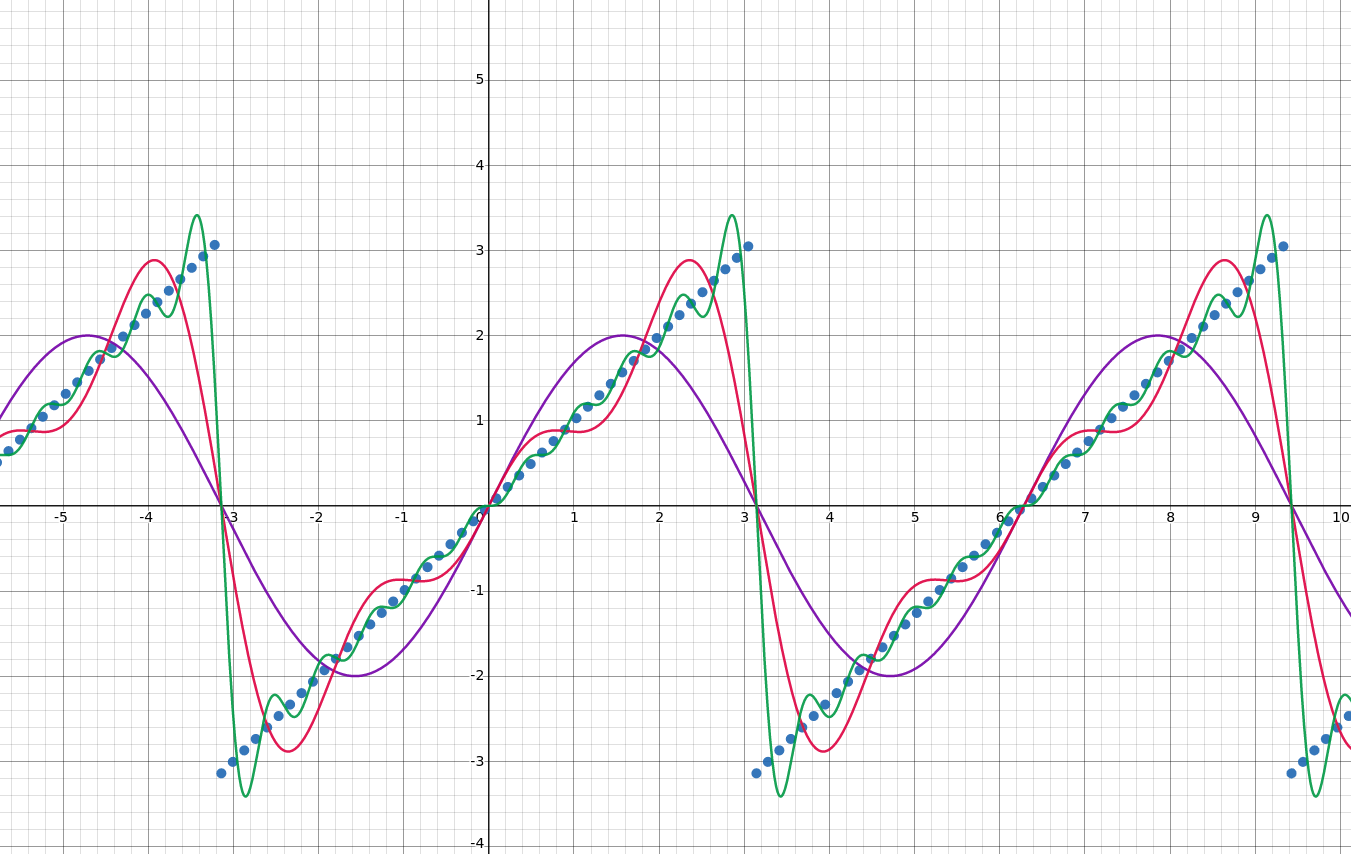
\includegraphics[width=\linewidth]{fourier_x.png}

                  \item Where does the Fourier series of $f$ converge? To what does
                        it converge?
                        \medbreak
                        The fourier series converges to $f(x)$ on $(-\pi, \pi)$ and
                        to $0$ at $\pm\pi$.
                  \item Show that the solution of the heat equation discussed in
                        problem 5 of section 9.1 satisfies the initial condition
                        at all $x\in[0,\pi]$ except $x=\pi$.
                        \medbreak
                        The fourier series converges to $f$ for all $x\in[0, \pi)$
                        but it does not converge at $\pi$.
            \end{enumerate}
            \setcounter{enumi}{6}
      \item Let $f$ be a twice continuously differentiable $2\pi$ periodic
            function. Prove that the Fourier series of $f$ converges to $f$
            uniformly.
            \begin{proof}
                  Since $f$ is continuous and periodic, we know there exists some $M>\lVert f(x)$ for all $x\in\mathbb{R}$.
                  % TODO: Finish this proof
            \end{proof}
            \setcounter{enumi}{9}
      \item A subset $E\subseteq \mathbb{R}$ is said to have \textbf{measure zero}
            if, given any $\varepsilon>0$, there is a countable family of intervals
            $\{I_n\}_{n=1}^\infty$ such that $E\subseteq\cup I_n$ and
            $\sum length(I_n)\leq \varepsilon$.
            \begin{enumerate}
                  \item Show that any finite set of points has measure zero.
                        \begin{proof}
                              Let $N$ be the number of points, and $\varepsilon>0$.
                              Then we can choose $\delta=\frac{\varepsilon}{N+1}$
                              and create an interval around each point
                              $I_n=(p_n-\frac{\delta}{2}, p_n+\frac{\delta}{2})$.
                              Then $\sum length(I_n)<\varepsilon$.
                        \end{proof}
                  \item Show that the set $\left\{\frac{1}{n}\right\}$ has measure zero.
                        % TODO: I don't understand what that set means
                  \item Show that any countable set has measure zero. Remark:
                        There are uncountable sets of measure zero.
                        \begin{proof}
                              Let $\varepsilon>0$, and $S_n$ be the subset of set $S$
                              which contains $n$ of its elements. Then we can choose
                              $\delta=\frac{\varepsilon}{n+1}$ and create an interval
                              $I_n=(p_n-\frac{\delta}{2}, p_n+\frac{\delta}{2})$ around
                              each point. Then $\sum length(I_n)<\varepsilon$. Suppose
                              that we allow $n\to\infty$. Then the equations above still
                              hold, and $\sum length(I_n)<\varepsilon$.
                        \end{proof}
            \end{enumerate}
\end{enumerate}

\subsection{Mean-square Convergence}

\begin{enumerate}
      \setcounter{enumi}{1}
      \item Let $\{f_n\}$ be a sequence of continuous functions on $[a,b]$ that
            converges to a function $f$ uniformly. Prove that $f_n\to f$ in the
            mean-square sense.
            \begin{proof}

            \end{proof}
      \item Let $[a,b]$ be a finite interval.
            \begin{enumerate}
                  \item Construct a sequence of continuous functions on $[a,b]$,
                        $\{f_n\}$, so that $f_n\to 0$ pointwise but
                        $\lVert f_n\rVert_2\to\infty$.
                  \item Construct a sequence of continuous functions on $[a,b]$,
                        $\{f_n\}$, so that $\lVert f_n\rVert_2\to\infty$ but
                        $\{f_n(x)\}$ does not converge to 0 for any $x\in[a,b]$.
            \end{enumerate}
            \setcounter{enumi}{5}
      \item \begin{enumerate}
                  \item Let $f$ be a piecewise continuous function on $[\pi,\pi]$.
                        Prove that there is a sequence of continuous functions
                        $f_n$ on $[\pi,\pi]$ so that $f_n\to f$ in mean-square sense.
                  \item Use the idea of the proof of theorem 9.4.6 to show that
                        the Fourier series of a piecewise continuous function $f$
                        converges to $f$ in the mean-square sense.
            \end{enumerate}
            \setcounter{enumi}{8}
      \item Let $f$ be a continuously differentiable function on $[-\pi,\pi]$
            such that \\$\int_{-\pi}^\pi f(x)dx=0$. Prove that
                  \begin{equation}
                        \int_{-\pi}^\pi \lvert f'(x)\rvert^2dx
                        \geq \int_{-\pi}^\pi \lvert f(x)\rvert^2dx.
                        \label{eq:9.4_9_given}
                  \end{equation}
                  Prove that strict equality holds in \eqref{eq:9.4_9_given} if and
                  only if $f(x)=a\cos x+b\sin x$ for some constants $a$ and $b$.
\end{enumerate}

\end{document}